\chapter{System Design and Architecture}\label{chap:design}
The following chapter describes the system's basic design and its program flow. As this project is partly an extension of an implementation of PSO \cite{haskellPSO}, Section~\ref{sec:original_pso_implementation} outlines the core architecture of that implementation in order to provide a base to the changes made in this project. Section~\ref{sec:expansion_for_portfolio_optimisation} explains the design and ideas behind the system's modification and further design on how to apply the algorithm to solve the portfolio optimisation problem.

  \section{Original PSO Implementation} % (fold)
  \label{sec:original_pso_implementation}
    \subsection{Initialisation} % (fold)
    \label{sub:initialisation}
    The main purpose of this stage is to create a population of particles (called a swarm) which will be used to search the domain and find the optimal solution to our problem. The application uses a function called \textit{initialise} to randomly create a list of initial particles to populate the search space. It is written in accordance with Algorithm~\ref{eq:pso} and thanks to Haskell's well designed and efficient random generators \cite{random} it ensures that the particles are initialised in such a way to exploit the search space well. For details, see Algorithm~\ref{eq:pso}. After the population has been initialised, the algorithm moves on to the optimisation phase.
    % subsection initialisation (end)
    \subsection{Inertia Weights} % (fold)
    \label{sub:inertia_weights}
    PSO relies on randomness, as in Equation~(\ref{eq:vel}). As this project is not intended to experiment much with the basic PSO parameters we will use the inertia weights presented in \cite{constriction_factor_3}. If there is enough time, we may wish to experiment with different weights. This does not mean that testing will not be done, it just means that we will not deviate from our goal to look into this matter, as so much research has already been done\cite{inertia}.
    % subsection inertia_weights (end)
    \subsection{Optimisation} % (fold)
    \label{sub:optimisation}
    This is done by ``steps'', at each ``step'' a particle is updated by a function \textit{updateParticle} in accordance to Equation~(\ref{eq:vel})which changes the position and velocity. The same function checks whether the new position is better that the best solution so far. A boolean system is used, if the new position of the particles is better that global best position, if it is then it changed the global best to this new global best. This is done recursively until all the particles in the swarm have been updated. Function had to be created to deal with the comparison of particles' results and both the position and the value of that position are stored for each particle. 

    For any more details on how the optimisation is done, please refer to \nameref{sec:particle_swarm_optimisation} in Chapter 2.
    % subsection optimisation (end)
    \subsection{Termination} % (fold)
    \label{sub:termination}
    A function was created to deal with the termination, a user specifies the number of iterations (``steps'') that the algorithm is allowed to run for. This independent function is simple, it runs recursively, applying one \textit{updateParticle} at a time and terminates once there are no more iterations to be performed and returns both the value of the global best and its position. 
    % subsection termination (end)
  % section original_pso_implementation (end)

  \section{Expansion for Portfolio Optimisation} % (fold)
  \label{sec:expansion_for_portfolio_optimisation}

    \subsection{Interface and User Input} % (fold)
    \label{sub:interface_and_user_input}
    The original implementation needed the swarm size and number of iterations to be hard-coded into the algorithm. This model allows the user to specify how many particles they would like as well as how many iterations the PSO should run for. I do not think the user should be allowed to set the inertia weights as they might not fully understand their purpose and therefore give non-optimal inputs.
    % subsection interface_and_user_input (end)
    \subsection{Data file} % (fold)
    \label{sub:data_file}
    The user will have to input a file with the assets' information in order for the system to optimise a portfolio. There is no standard format for such a file and it really is up to preference. I have decided to arrange the file as follows: ``Name Rate-Of-Return Expected-Required-Return'', where \textit{Name} is the companies name (either full or just the ticker), \textit{Rate-Of-Return} is the rate of return for the company and \textit{Expected-Required-Return} is the expected required return of the same company with each company on a different line. 

    Figure~\ref{fig:asset_file} shows an example file containing a selection of assets which the user wants to maximise for their portfolio. As you can see the first item is the name of the company, followed by a single space and then the rate of return, another space and the expected return. Each company has their own line and they can have as many companies as they would like. 
    \begin{figure}[H]
      \centering
        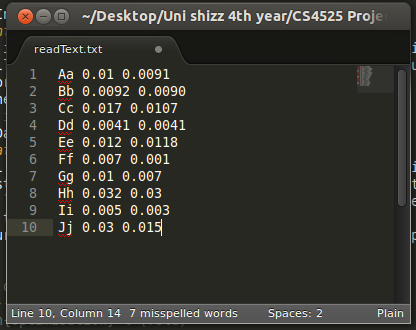
\includegraphics[width=0.9\textwidth]{asset-file}
      \caption{Example File of Assets.}
      \label{fig:asset_file}
    \end{figure}
    % subsection data_file (end)
    % ----------------------------------------------------
    % \subsection{Optimisation} % (fold)
    % \label{sub:optimisation}
    
    % % subsection optimisation (end)
    % ----------------------------------------------------
    \subsection{Constriction Factor} % (fold)
    \label{sub:constriction_factor}
    Maurice Clerc in his study on stability and convergence of PSO \cite{constriction_factor} has introduced the concept of a constriction factor. Clerc indicated that the use of a constriction factor may be necessary to insure convergence of the PSO for certain fitness functions.

    In order to ensure convergence of the PSO, the velocity from Equation~(\ref{eq:vel}) can be expressed as follows:
    \begin{equation} \label{eq:cf}
      \begin{split}
        V_{i}^{t+1} & = K \Bigg[ V_{i}^{t} + c_1 r_1 \times \Big( Pbest_{i}^{t} - X_{i}^{t} \Big) + c_2 r_2 \times \Big( Gbest^{t} - X_{i}^{t} \Big) \Bigg] \\
        \text{where }\\
        K & = \frac{2}{\mid 2 - \phi - \sqrt{\phi^2 -4\phi} \mid} \text{ and } \phi = c_1 + c_2 \text{ s.t. } \phi > 4  \\
        % \text{and} \\
        % \phi = c_1 + c_2 , \phi > 4 \\
      \end{split}
    \end{equation}

    The convergence characteristic of the system can be controlled by $\phi$ through choosing suitable $c_1$ and $c_2$ in \eqref{eq:cf}. In this approach, $\phi$ must be greater than 4 to guarantee stability \cite{constriction_factor_2}.
    % subsection constriction_factor (end)
    \subsection{Termination} % (fold)
    \label{sub:termination}
    If time allows, it would be nice to have a self-termination PSO which, no matter how many iterations are left, terminates if it thinks that the optimal solution is reached. This could be done by the concept of a threshold, if all the solution reach this threshold, then there is no point in carrying on. For example, if all the solution are close enough to each other for a long period of iteration, say $10^{-10}$, then there is no point in looking for thousands more iterations just to find something which will not affect the outcome. 

    In order to achieve this, we would need three extra parameters to be added, one to define the threshold, another one to define the maximal number of iterations allowed without improvement (call this \textit{mni}, and another one to compute the current number of remaining iterations allowed without improvement(call this \textit{cni}. After each call to the updating function, compare the current best solution to the past best solution to decide whether there has been a relevant improvement or not. The algorithm would either change the number of iterations to \textit{mni} (in case there was relevant improvement), otherwise reduce the value of \textit{cni} by one. 
    % subsection termination (end)
    \subsection{Fitness Function} % (fold)
    \label{sub:fitness_function}
    Due to the nature of Haskell and with some mathematical background it is almost trivial to create a function to represent the measure of risk, namely $\rho_{a,p}(R)$ in Equation~(\ref{eq:portfolio-risk}) in Section~\nameref{sec:portfolio_management} Chapter~\ref{chap:background}. What is much more challenging is finding a way to include the constraints in Equation~(\ref{eq:portfolio-risk-constraints}) in a way that the algorithm can deal with the main function without violating these condition. Two methods were considered, using multi-objective optimisation or a penalty function. Due to the constraints being linear-independent, it will be straight forward to affect the optimal solution through factors of the constraints. The design of this will be described in the following Subsection~\ref{sub:penalty_function}.
    % subsection fitness_function (end)
    \subsection{Penalty function} % (fold)
    \label{sub:penalty_function}
    One of the most straight forward approaches to solving constrained optimization problems is the use of a penalty function\cite{constraint}. Using such an approach means transforming the optimisation problem, such our $\rho_{a,p}(R)$ in Equation~(\ref{eq:portfolio-risk}), to include the behaviour of being ``punished'' if the constraints are not met. One can construct a single new objective function from combining $\rho_{a,p}(R)$ plus linear factors of each constraint in Equation~(\ref{eq:portfolio-risk-constraints}), this new objective function will be used to find an optimum value for the portfolio problem. Thus a new optimisation function can be created:
      \begin{equation} \label{eq:unconstraint-portfolio-risk}
        \begin{split}
          \text{min } f(R) & \\
          \text{where } 
          f(R) & = \rho_{a,p}(R) + \frac{1}{\delta}|\widehat{R}-\eta| + \frac{1}{\delta}|\sum\limits_{i=1}^N x_i -1| \\
          % \rho_{a,p}(R) & = a \|(R-\widehat{R})^+\|_1 + (1-a)\|(R-\widehat{R})^-\|_p - \widehat{R} \\
        \end{split}
      \end{equation}
    Now an explanation on what is happening in Equation~(\ref{eq:unconstraint-portfolio-risk}). Firstly,$\delta > 0$ is called the penalty parameter and $\frac{1}{\delta}$ is called the penalty value \cite{constraint}. The penalty parameter should be small enough so that whenever a constraint is violated, the penalty value will be big enough to affect the result to the solution. Secondly, the use of absolute values refers to the distance traveled from the desired value, for example if the sum of the weights is not equal to 1 then $|\sum\limits_{i=1}^N x_i -1| > 0$ multiplying this by a penalty value will be ensure that the solution will not be taken as an optimal one. Finally, similar method in used for deviating from the required expected return. 

    One may notice that in this new optimisation function, the lower and upper bounds for how much one can invest in each asset is not included. This is due to how PSO handles search space domains and will be explained in the following Subsection~\ref{sub:forced_diversification}.
      % \begin{equation} \label{eq:portfolio-risk}
      %   \begin{split}
      %     \rho_{a,p}(R) & = a \|(R-\widehat{R})^+\|_1 + (1-a)\|(R-\widehat{R})^-\|_p - \widehat{R} \\
      %   \end{split}
      % \end{equation} 
      % Now that there is a way to measure risk, the portfolio optimisation problem can be formulated as follows:
      % \begin{equation} \label{eq:portfolio-risk-min}
      %   \begin{split}
      %     \text{min } \rho_{a,p}(R) \\
      %   \end{split}
      % \end{equation} 
      % Subject to constraints:
      % \begin{equation} \label{eq:portfolio-risk-constraints}
      %   \begin{split}
      %     \widehat{R} = \eta \\
      %     \sum\limits_{i=1}^N x_i = 1 \\
      %     l_i \leq x_i \leq u_i
      %   \end{split}
      % \end{equation}
    % subsection penalty_function (end)
    \subsection{Forced Diversification} % (fold)
    \label{sub:forced_diversification}
    Equation~(\ref{eq:unconstraint-portfolio-risk}) did not include lower and upper limits for each assets as in Equation~(\ref{eq:portfolio-risk-constraints}), this is because the implementations \cite{haskellPSO} already takes into account bounds for the solutions' domain for a given fitness function. Since our objective is to find weights for each asset, the set of assets is the domain for our fitness function. So the bounds for the proportions can be set which the algorithm.

    The bounds inside PSO can be used to give a sense of diversification \cite{diversification}, by not allowing how much you invest on each asset to be too small or to large. For example, you might specify that you have to invest at least 5\% and at most 50\% of any asset in a portfolio, this forces the investor to consider at all assets and helps lowering the risk of a portfolio \cite{diversification}.
    
    % subsection forced_diversification (end)
    \subsection{Presenting the Results} % (fold)
    \label{sub:presenting_the_results}
    After the algorithm has finished, the results are displayed on the screen and saved in a separate file which will be called ``output-DATE'', where date is in (year,month,day) format, for example ``output-2014,3,15''. If there is multiple runs in one day, the new results are added to the end of that same file.
    % subsection presenting_the_results (end)
  % section expansion_for_portfolio_optimisation (end)


% \chapter{Financial Data}
%   \section{Data Description} % (fold)
%   \label{sec:data_description}
  
%   % section data_description (end)

%   \section{Problem Domain} % (fold)
%   \label{sec:problem_domain}
  
%   % section problem_domain (end)

%   \section{Assets and their Weights} % (fold)
%   \label{sec:assets_and_their_weights}
  
%   % section assets_and_their_weights (end)

%   \section{Analysis} % (fold)
%   \label{sec:analysis}
  
%   % section analysis (end)

%   \section{PSO Parameters} % (fold)
%   \label{sec:pso_parameters}
  
%   % section pso_parameters (end)

%   \section{Experimentation and Testing} % (fold)
%   \label{sec:experimentation_and_testing}
  
%   % section experimentation_and_testing (end)

%   \section{Portfolio Constraints} % (fold)
%   \label{sec:portfolio_constraints}
  
%   % section portfolio_constraints (end)

%   \section{Results} % (fold)
%   \label{sec:results}
  
%   % section results (end)
